\chapter{Experimental Setups}
\label{cap:setup}

\textit{In this chapter the experimental setups used will be shown and explained in detail.}

\section{Introduction}

The experimental setups used in this work had two main themes: droplets on heated surfaces and pool boiling. In the Droplets Experiments a vertical and horizontal view were considered, but in the boiling experiments, because of the water opacity to IR radiation, only the vertical experiment was made.


\section{About the IR Camera}
\label{sec:icam}
The IR Camera, an Onca-MWIR-InSb from Xenics, is the main device used in this dissertation and its function is to give an "image" of the analyzed object's temperature field. Its 2D array of sensors reads the incident IR radiation. Its signal is then converted to temperature in the camera's software. The user will end up with a bi-dimensional field of temperatures with a +/- 0.5ºC precision. This camera can be seen in Figure \ref{fig:onca}.

\begin{figure}[h!]
\centering
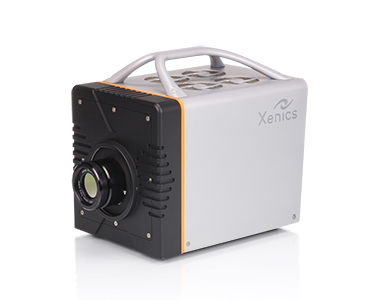
\includegraphics[width=0.6\linewidth]{Figures/2.Chapter/onca.png}
\caption{Xenics' Onca-MWIR-InSb}
\source{http://www.xenics.com/en/onca-mwir-insb}
\label{fig:onca}
\end{figure}

\subsection{Camera properties}

\par The relevant properties of the Onca-MWIR-InSb can be seen in Table \ref{tab:camprop}.

\begin{table}[h]
\centering
\caption{Camera Properties}
\label{tab:camprop}
\begin{tabular}{lclclc}
\toprule
\multicolumn{2}{c}{Camera Characteristics} & \multicolumn{2}{c}{Optical System} & \multicolumn{2}{c}{Image Characteristics} \\
\cmidrule[0.4pt](r{0.125em}){1-2}%
\cmidrule[0.4pt](r{0.125em}){3-4}%
\cmidrule[0.4pt](r{0.125em}){5-6}%
Sensor                 & InSb (MWIR)       & Focal lens          & 13 mm        & Video Rate         & 60Hz                 \\
Spectral Sensibility   & 3.5-5 $\mu m$     & Optics Material     & Germanium    & Max framerate      & 3000 fps             \\
Spatial Resolution     & $320 \times 256$  &  -                  & -            & Min pixels (ROI)   & $15 \times 5$        \\
Thermal Sensibility    & \textless17mk     &   -                 &   -          & Exposition         & \textgreater 1 $\mu s$  \\ \bottomrule
\end{tabular}
\end{table}


\subsection{The Software}

\par This camera has its own specific software, Xeneth, which will be very important throughout this work. It's relevant to explain its functioning, which will be referenced various time in this dissertation.

\subsubsection{Selecting a Calibration Pack}

\par When the program is executed a menu will appear. In this menu it's possible to select not only the used camera (there is also an option to select a virtual camera, used to play previously recorded videos) but also to select a calibration pack as it is shown in Figure \ref{fig:consetup}.
\begin{figure}[h]
\centering
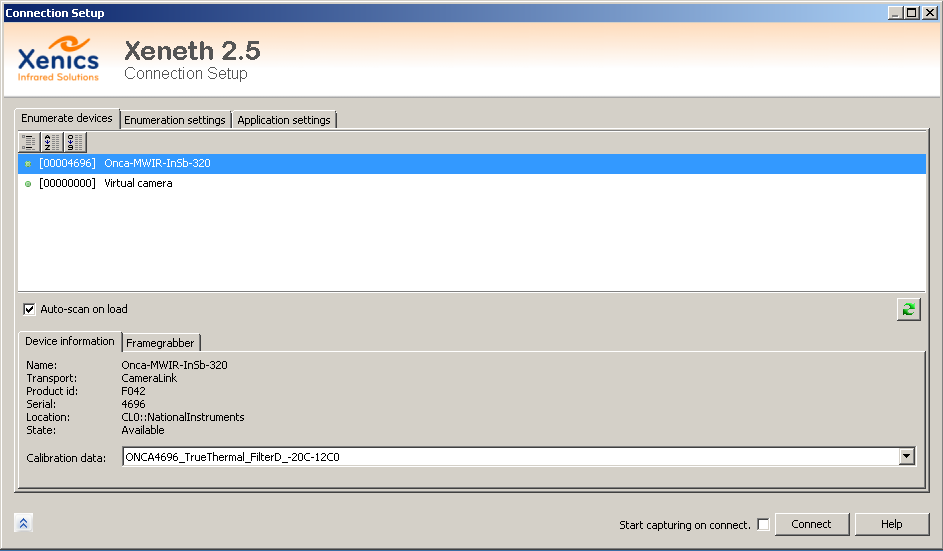
\includegraphics[width=0.7\linewidth]{Figures/3.Chapter/xeneth1.png}
\caption{Xeneth: Connection Setup Menu}
\label{fig:consetup}
\end{figure}
\par In the Calibration data drop menu are available several calibration packs. The main packs are:
\begin{itemize}
\item TRUE NUC: This pack is the one chosen if one wants to get data without temperature conversion. It presents results in ADU (received signal intensity) and it's adaptable to any integration time
\item TRUE THERMAL: This pack comes with a factory made calibration, so the results are presented in Celsius. This is used if the user just pretends a low thermal resolution measure or a qualitative result. It measures temperatures from -20 to 120ºC in any integration time.
\item User Calibration Packs: The user may want to create his own pack adapted to his own temperature interval, to use in a more precise application.
\end{itemize}

\subsubsection{Main Window}
\label{software}
\par After choosing the right calibration for the desired application and before starting the measurements, one should adjust several parameters in the main software window. The displayed panels can be shown in Figure \ref{fig:xeneth2}. There is a panel for the Camera Image, where one can see the thermal image and select an area or dot to take its read value and other statistics; a User Interaction Panel, where one can change settings, view and set the selection properties, record and save videos and choose image filters; a panel that shows the plotted measured data. In the right side we can also see a colour bar. This bar is adjustable so that we can adapt the colour gradient to the desired temperature interval to better observe the phenomena. \\
\begin{figure}[h]
\centering
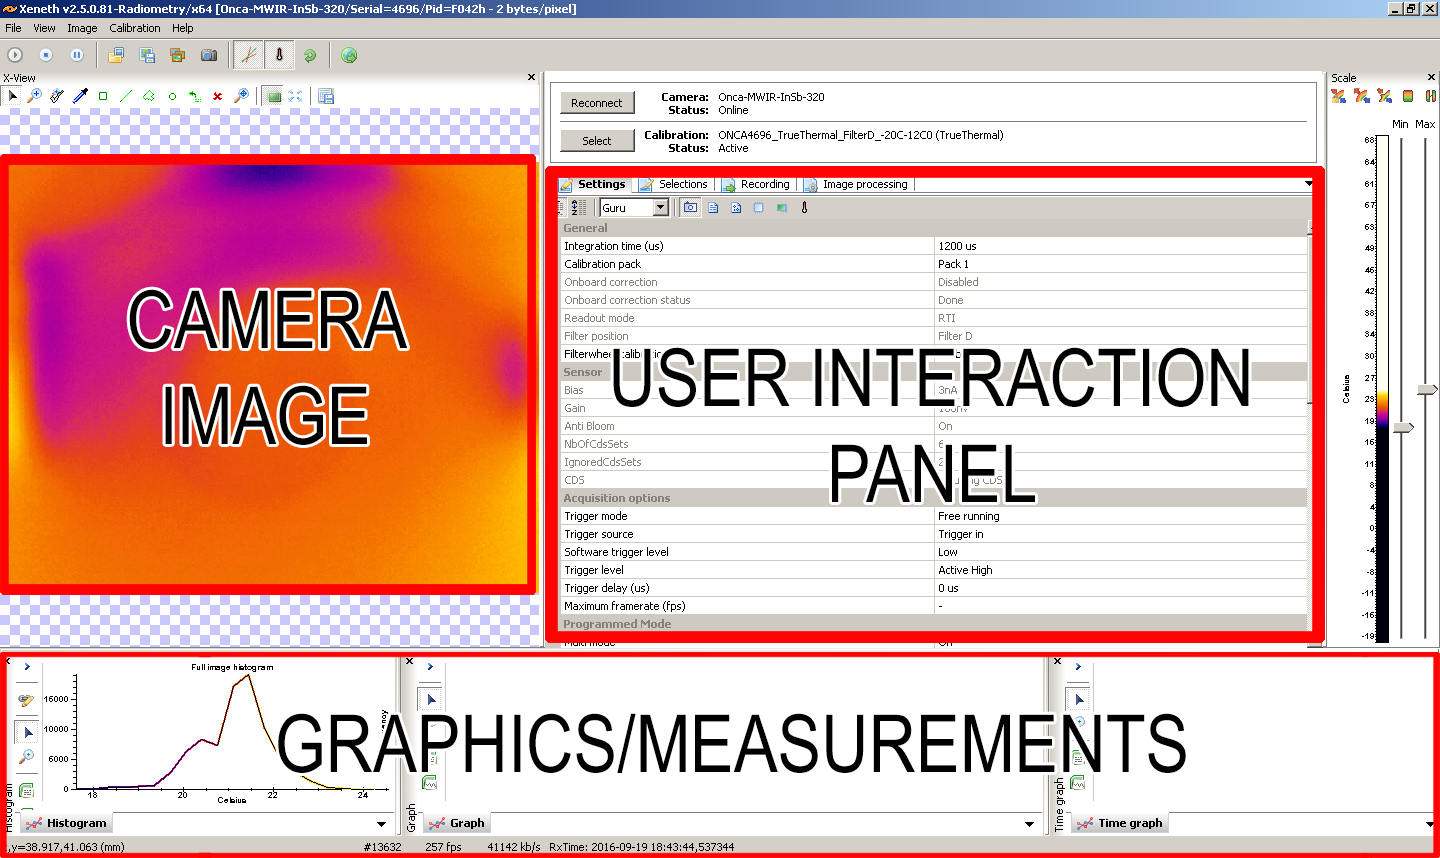
\includegraphics[width=0.7\linewidth]{Figures/3.Chapter/xeneth2.png}
\caption{Xeneth: Main Window Scheme}
\label{fig:xeneth2}
\end{figure}
\par Before starting there are some important settings to review to assure the best image possible. These parameters can be altered in the User Interaction Panel. The first and one of most important parameters is the integration time. The integration time can be easily explained as the equivalent to a common camera's exposure. If we increase the integration time we increase the sensitivity and reduce the noise. On the other side the image will saturate easier, which means that the temperature range highly decreases. So if a higher temperature range is needed, one should decrease the integration time until the desired range is obtained. Increasing the integration time will also affect the frames-per-second (fps) which may not be relevant for static measurements, but the phenomena studied in this dissertation requires high time precision because they happen in the order of milliseconds. The next important value we should consider is the Ambient Temperature and the Atmospheric Temperature. We can also alter this in the User Interaction Panel. To figure out the Ambient Temperature a highly reflective object is put in front of the camera and its temperature measured considering the body to be black. \\
\par The measurements can be made using the Selection Panel, present in Figure \ref{fig:xeneth3}. In this panel it is possible to select a shape (a circle in the case presented) and gather the statistics about the temperature in that area, including average, spatial and temporal deviation. It is also using this method that the temperature of the observed object is measured in this work as it is explain further ahead. Another function in this panel is the Zoom function. It is very important to restrict the measured area as much as it is possible with this function, in order to increase the frames-per-second. \\
\begin{figure}[h]
\centering
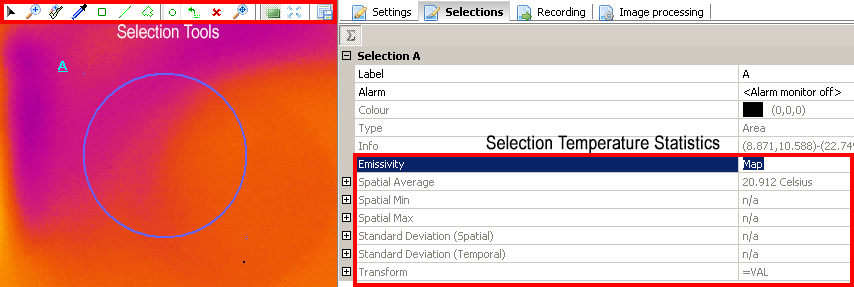
\includegraphics[width=0.7\linewidth]{Figures/3.Chapter/xeneth3.png}
\caption{Xeneth: Selection Panel}
\label{fig:xeneth3}
\end{figure}
\subsubsection{Offset Calibration}
\par When the user selects any of the factory calibrations, there is something that may not seem right. A simple blackbody with constant temperature may appear to have temperature variations as it can be seen in the left of Figure \ref{fig:xeneth5}. This happens due to the Dionisio effect. The Dionisio effect is the reflection of the camera on itself and it is a great error source, so it needs to be eliminated. \\
\begin{figure}[h]
\centering
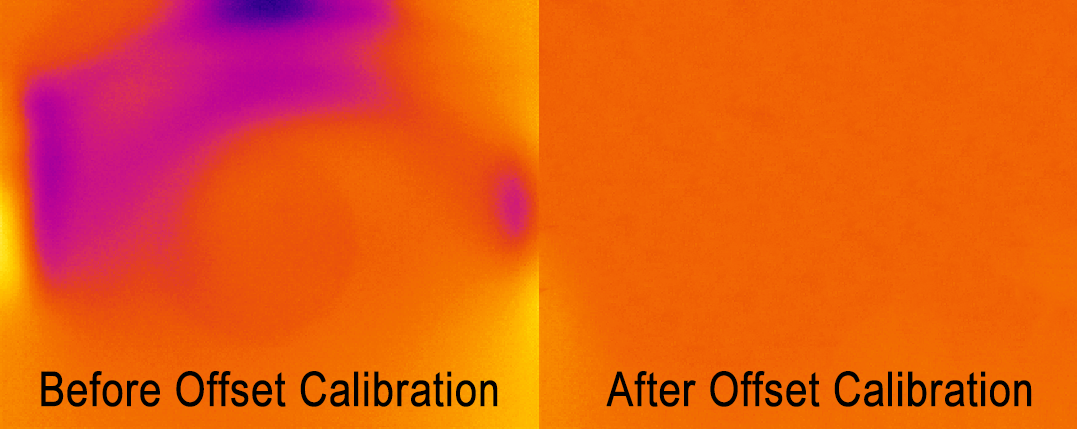
\includegraphics[width=0.7\linewidth]{Figures/3.Chapter/xeneth5.png}
\caption{Offset Calibration: Before and After}
\label{fig:xeneth5}
\end{figure}
\par A good way to eliminate this error is to use a software tool: the Offset Calibration. This can be found in the Calibration Wizard (a menu of calibration options for the camera) and has a simple function. It averages the temperature in space and time and sets every pixel to read that temperature. This eliminates the camera's reflection and also part of the noise and bad pixels. A disadvantage of this method is that it sometimes creates lesser periodic noise, which can be a problem to the measurements. The code behind this function is unknown, so the noise source could not be detected and could only be attenuated later in the post-processing stage. The result of the Offset Calibration can be seen in the right side of Figure \ref{fig:xeneth5}. \\

\section{Droplet Horizontal View}

\par The main objective of this experiment was to observe qualitatively the heat gradients in the droplet as it collides with the heated surface and removes its heat. To create a heater, cartridge resistance heaters were put under an aluminum plate, radiating to its surface. The experiment was made for water droplets, and the surface was hydrophilic. \\

\par To minimize the surface roughness interference a silica wafer was used, thus assuring a droplet fall as symmetric as possible. In the interface of the silica wafer and the aluminum plate a thermal paste was used to improve heat transfer. On top of the silica wafer there is a thermocouple that tracks the surface temperature. This setup can be seen in detail in Figure \ref{fig:horizontal2}. The thermocouple value is used by a PID controller to control the heat released by the cartridge heater. In the PID's screen the temperature of the plate is at its top and the target temperature at the bottom.\\

\begin{figure}[h]
\centering
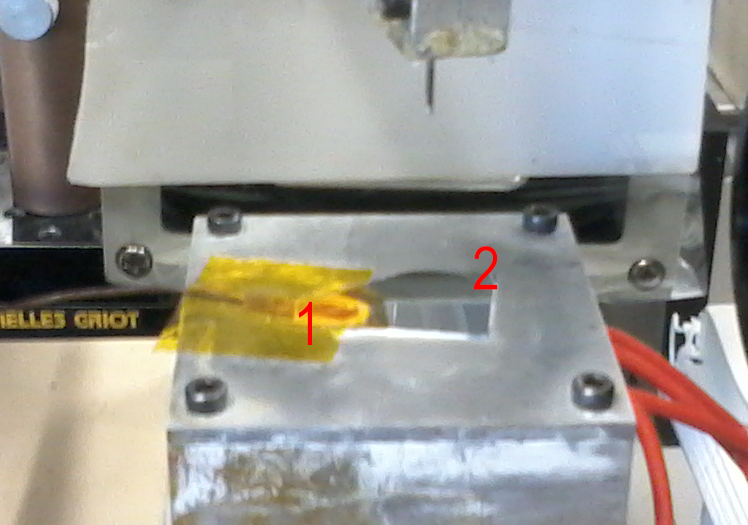
\includegraphics[width=0.5\linewidth]{Figures/3.Chapter/horizontal2.png}
\caption{Silica wafer setup: (1) Thermocouple, (2) Silica Wafer}
\label{fig:horizontal2}
\end{figure}

\par An Harvard Apparatus controls a syringe's water discharge, that then falls from the needle to the wafer. This forms a droplet with 2.6 to 3 mm diameter spherical droplet. This experiment is recorded by 2 cameras: IR camera and high-speed camera. In order for the high-speed camera to work, a high intensity lamp is also needed. The described setting can be seen in Figure \ref{fig:horizontal}. This setting was used to gather qualitative results only. Good quantitative results are impossible due to the implications of droplet geometry in thermography.

\begin{figure}[h]
\centering
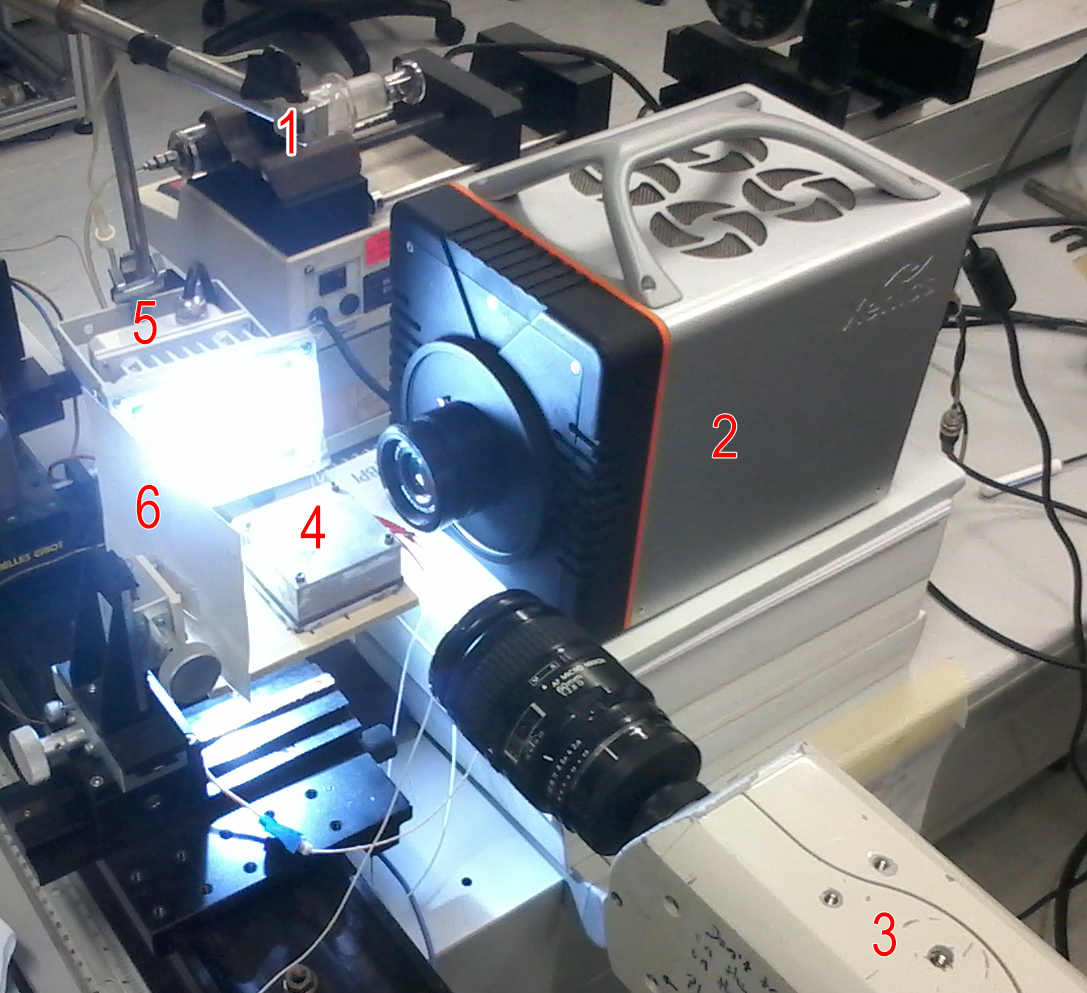
\includegraphics[width=0.65\linewidth]{Figures/3.Chapter/horizontal.png}
\caption{Horizontal setup: (1) Needle, (2) IR Camera, (3) HS Camera, (4) Heated Surface, (5) Lamp, (6) Black Background}
\label{fig:horizontal}
\end{figure}

\subsection{Procedure}
\label{sec:procedure}
\begin{itemize}
\item Adjust IR Camera's settings on the software.
\item Perform an offset calibration (described in Section \ref{sec:icam}).
\item Adjust PID controller to the desired temperature and water flow in the Harvard Apparatus.
\item Turn on the light and set the cameras recording.
\item Let a droplet drop on the wafer.
\item Clean the wafer with acetone and distilled water before proceeding.
\end{itemize}

\section{Droplet Bottom View}

\par The objective of this setup is to observe interface temperatures in during the droplet impact phases. To do this, the IR Camera had to be placed underneath the surface in which the droplet impacts. The droplet impacts on a 20 $\mu m$ thick stainless steel foil. This was done similarly to \cite{sielaff2014experimental}, as the objective was to read the interface temperatures. Because of the small thickness of the foil, the temperature of the interface is very similar to the read temperature in the bottom of the foil. The HS camera was placed horizontally to the foil to observe the impact. A lamp was placed in the opposite site. The setup scheme can be seen in Figure \ref{fig:setup}.\\

\begin{figure}[h]
\centering
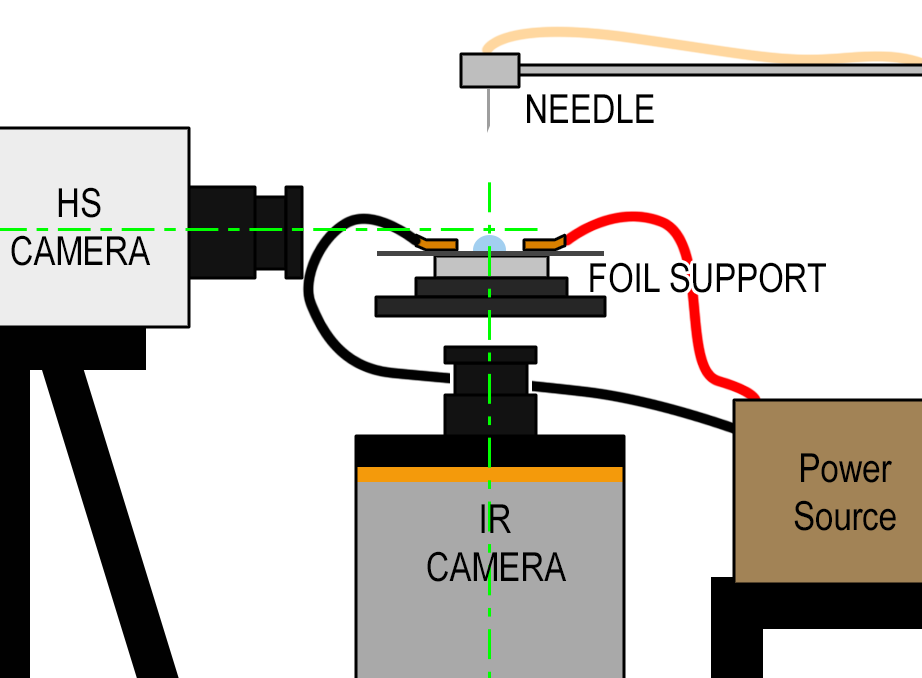
\includegraphics[width=0.55\linewidth]{Figures/3.Chapter/setup.png}
\caption{Bottom Setup Scheme}
\label{fig:setup}
\end{figure}

\par The experiments made around this setup were made using hydrophilic (using distilled water and ethanol) and super-hydrophobic (using just water) surfaces. A preliminary experiment with water and an hydrophilic surface was made, using the software calibration. From the first, raw results were taken for posterior calibration and processing. The calibrations and their differences are explained in Chapter \ref{cap:setup}.\\

\par The foil is fed an electric current, so it can heat up to the desired temperature. This is done by to electrical contacts, wired to a power source. The foil has to be placed on top of a bad heat conductor to minimize heat losses. A heat glass was chosen for the purpose. It also needs to be stretched so that possible wrinkles don't affect the droplet. A detail of the setup, on the foil support can be seen in Figure \ref{fig:suporte}. In this figure two supports are shown. The second was made after the calibration. \\

\par For the case of the super-hydrophobic surfaces, the surfaces needed to be cleaned with an ultra-sound bath and coated with \textit{Glaco}. This coating took several layers to ensure effective coating that can endure high temperature and constant droplet fall. \\

\begin{figure}[h]
\centering
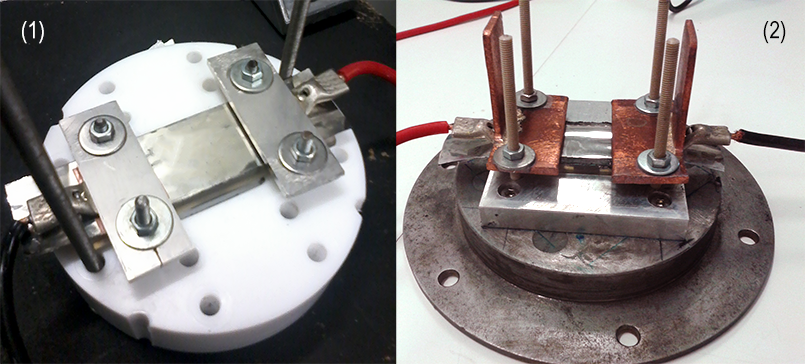
\includegraphics[width=0.9\linewidth]{Figures/3.Chapter/suporte.png}
\caption{Stainless Steel Support: (1) Before calibration setup, (2) After calibration setup}
\label{fig:suporte}
\end{figure}

\par This setup also has the Harvard Apparatus and the needle to create the droplet. A metal structure holds the support, needle and camera. The complete setup can be seen in Figure \ref{fig:setup2}. Although we have a different calibration, the procedure is similar to the previously described in \ref{sec:procedure}. The big difference is that the foil temperature is controlled with the power source and not with the PID. To adjust the current correctly one needs to read the temperature on the IR Camera's software. In the case that raw images are needed, an additional step should be to convert the desired temperatures in ADU. Only this way one can know if the foil is at the desired temperature.

\begin{figure}[h]
\centering
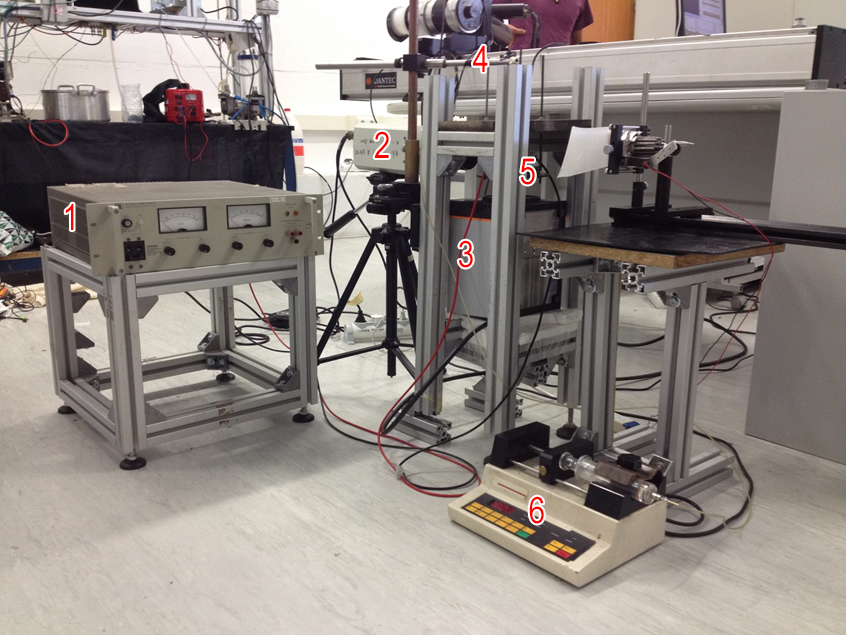
\includegraphics[width=0.9\linewidth]{Figures/3.Chapter/setup2.png}
\caption{Bottom Setup: (1) Power Source, (2) HS Camera, (3) IR Camera, (4) Needle, (5) Foil Support, (6) Harvard Apparatus}
\label{fig:setup2}
\end{figure}
%%\section{Section B}
\label{sec:sectionb}

\subsection{Subsection A}
\label{subsec:subasectionB}

The model described can also be represented as

\begin{equation}
\dot{\mathbf{x}}(t) = \mathbf{T}\mathbf{z}(y),\  \mathbf{y}(0) = \mathbf{y}_0,\  z\geq 0 \\
\label{eq:dummyeq1}
\end{equation}

\noindent where

\begin{equation}
\mathbf{A} = \left[ \begin{array}{cc} -(a_{12} + a_{10}) & a_{21} \\ a_{12} & -(a_{21} + a_{20}) \end{array} \right],\ \mathbf{x} = \left[ \begin{array}{c} x_1 \\ x_2 \end{array} \right] \\
\label{eq:dummyeq2}
\end{equation}


\subsection{Subsection B}
\label{subsec:subbsectionB}

\begin{table}[H]
	\centering
	\caption{Dummy Table.}
	\begin{tabular}{|c|c|c|c|} \hline
		\textbf{Vendor Name} 				& \textbf{Short Name}	& \textbf{Commercial Name}	& \textbf{Manufacturer}	\\ \hline \hline
		\multirow{3}{*}{Text in Multiple Row}		&	ABC				&  ABC\textreg				& ABC SA			         \\ \cline{2-4}
		 								&        DEF				&  DEF\textreg				& DEF SA				\\ \cline{2-4}
										&        GHF			&  GHF\textreg				& GHF SA				\\ \hline
		Text in Single Row					&        IJK				& IJK\textreg				& IJK SA				\\ \hline
		Frescos SA						&        LMN			& LMN\textreg				& LMN SA				\\ \hline
		Carros Lda.						&    \multicolumn{3}{|c|}{Text in Multiple Column}							\\ \hline
	\end{tabular}
	\label{tab:dummytable}
\end{table}
\cleardoublepage